\section{Evaluierung des Wellenfrontrekonstruktionsalgorithmus}

\subsection{Überblick}
\begin{frame}{Versuchsaufbau}
	\begin{tikzpicture}
		\node at (0,0) {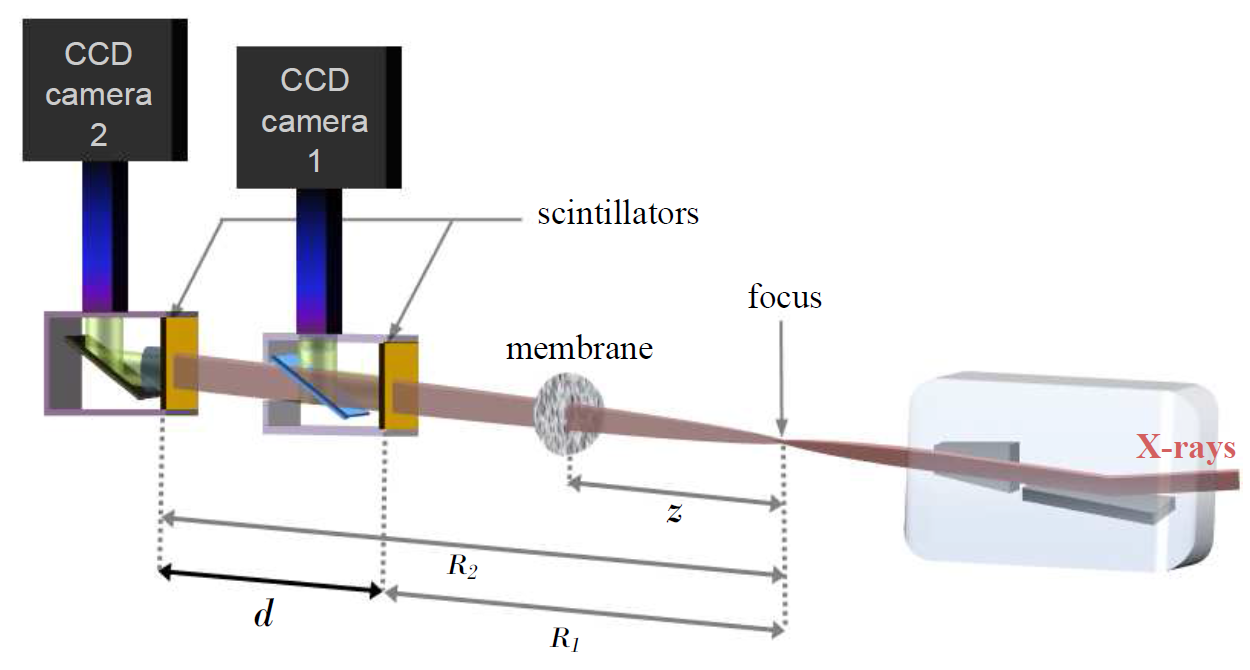
\includegraphics[width=0.98\linewidth]{./img/Versuchsaufbau.png}};
		\only<2>{\draw[red, very thick] (2.4, -2.2) rectangle (5.5, -0.2);}
		\only<3>{\draw[red, very thick] (1.2, -1.2) rectangle (1.6, -0.8);}
		\only<4>{\draw[red, very thick] (-1.1, -1.4) rectangle (0.3, 0);}
		
		\only<5>{\draw[red, very thick] (-5.5, 2.9) rectangle (-1.7, -1);}
		\only<6>{\draw[red, very thick] (-4.3, -2.7) rectangle (-2.1, -2);}
		\only<7>{\draw[red, very thick] (-3.3, -1) rectangle (-1.7, 0.1);}
		
		\only<8>{\draw[red, very thick] (-3.6, 1.2) rectangle (-1.9, 2.7);}
		\only<8>{\node at (3.4,0.8) {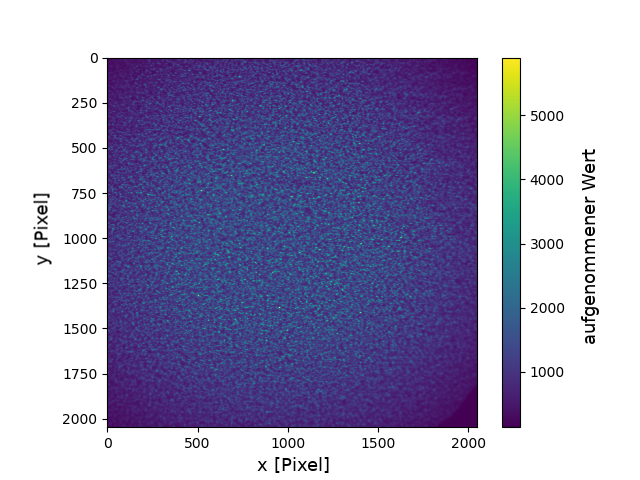
\includegraphics[width=0.5\linewidth]{img/ref_start0001_1-10}};}
		\only<8>{\draw[red, very thick] (0.7, 2.8) rectangle (6.0, -1.33);}
		\only<8>{\draw[red, very thick] (0.7, 2.8) -- (-1.9, 2.7);}
		\only<8>{\draw[red, very thick] (0.7, -1.33) -- (-1.9, 1.2);}
		
		\only<9>{\draw[red, very thick] (-5.3, -0.8) rectangle (-3.7, 0.3);}
		\only<10>{\draw[red, very thick] (-5.5, 1.5) rectangle (-3.8, 2.9);}
		
		\only<10>{\node at (3.4,0.8) {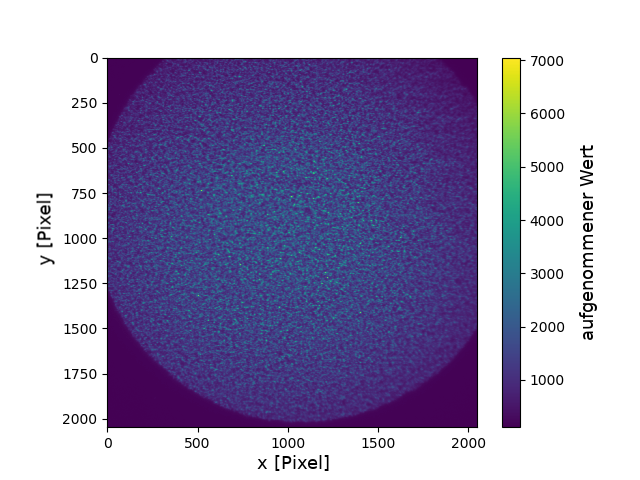
\includegraphics[width=0.5\linewidth]{img/E10001}};}
		\only<10>{\draw[red, very thick] (0.7, 2.8) rectangle (6.0, -1.33);}
		\only<10>{\draw[red, very thick] (0.7, 2.8) -- (-3.8, 2.9);}
		\only<10>{\draw[red, very thick] (0.7, -1.33) -- (-3.8, 1.5);}
	\end{tikzpicture}
	\nocite{Ber12}
	\nocite{Ber13}
	\nocite{Ber15}
	{\scriptsize \citeall{Ber15}}
\end{frame}

\begin{frame}{Überblick}
	\textbf{Hauptroutine:} 
	\begin{itemize}
		\item Korrigieren von Kamerafehlern
		\item Ablenkung nachverfolgen
		\item Wellenfront rekonstruieren
	\end{itemize}
\end{frame}

\begin{frame}{Hauptroutine}
	\only<1>{\vspace{-0.37cm}}
	\begin{tikzpicture}
		\node at (-5,0.6) {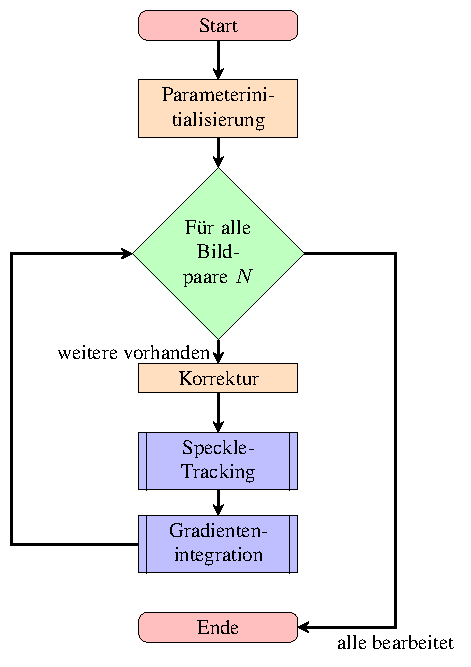
\includegraphics[width=0.4\linewidth]{pdf/graph_main}};
		\only<2-4>{\node at (-1,0) {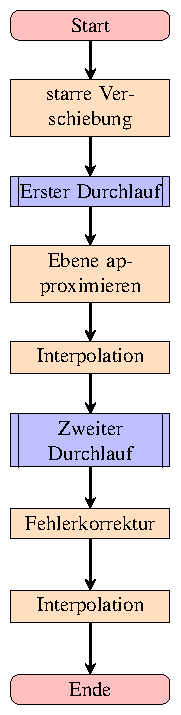
\includegraphics[width=0.17\linewidth]{pdf/graph_speckle}}};
		
		\only<2>{\draw[red, very thick] (-6.0, -1.0) rectangle (-4.3, -0.3)};
		\only<2>{\draw[red, very thick] (-4.3, -0.3) -- (-2, 3.8)};
		\only<2>{\draw[red, very thick] (-4.3, -1.0) -- (-2, -3.8)};
		\only<2>{\draw[red, very thick] (-2, -3.8) rectangle (0.0, 3.8)};
		
		\only<3-4>{\draw[red!25, very thick] (-6.0, -1.0) rectangle (-4.3, -0.3)};
		\only<3-4>{\draw[red!25, very thick] (-4.3, -0.3) -- (-2, 3.8)};
		\only<3-4>{\draw[red!25, very thick] (-4.3, -1.0) -- (-2, -3.8)};
		\only<3-4>{\draw[red!25, very thick] (-2, -3.8) rectangle (0.0, 3.8)};
		
		\only<3>{\draw[red, very thick] (-1.95, 1.5) rectangle (-0.0, 2.05)};
		\only<3>{\node at (2,0) {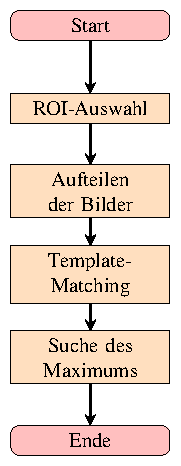
\includegraphics[width=0.17\linewidth]{pdf/graph_first_pass}}};
		\only<3>{\draw[red, very thick] (0.0, 2.05) -- (1, 2.5)};
		\only<3>{\draw[red, very thick] (0.0, 1.5) -- (1, -2.5)};
		\only<3>{\draw[red, very thick] (1.0, -2.5) rectangle (3.1, 2.5)};
		
		\only<4>{\draw[red, very thick] (-1.95, -1.25) rectangle (-0.05, -0.55)};
		\only<4>{\node at (2,0) {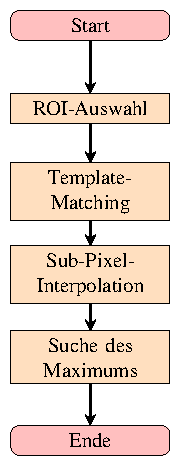
\includegraphics[width=0.17\linewidth]{pdf/graph_second_pass}}};
		\only<4>{\draw[red, very thick] (-0.05, -0.55) -- (1, 2.5)};
		\only<4>{\draw[red, very thick] (-0.05, -1.25) -- (1, -2.5)};
		\only<4>{\draw[red, very thick] (1.0, -2.5) rectangle (3.1, 2.5)};
		
		\only<5>{\draw[red, very thick] (-6.0, -1.0) rectangle (-4.3, -0.3)};
		\only<5>{\node at (1,2.2) {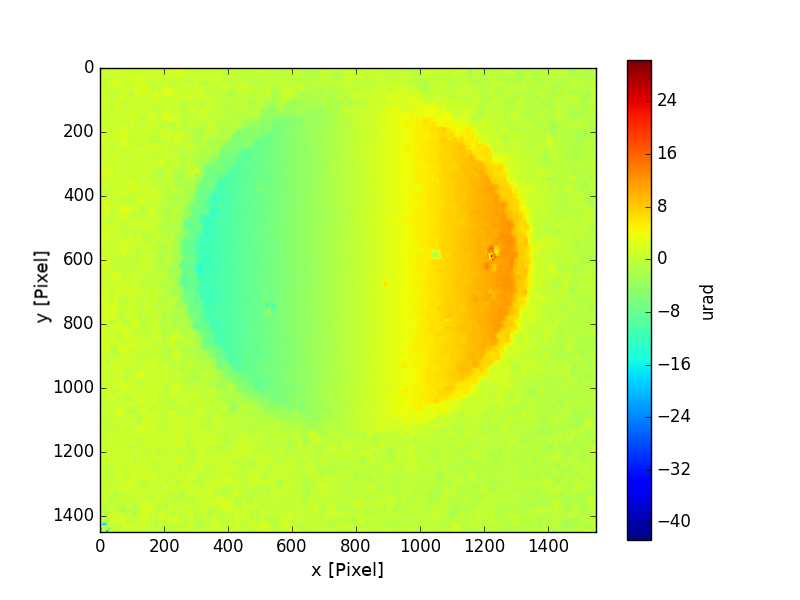
\includegraphics[width=0.38\linewidth]{img/SpeckDisH_E10001_edf_ref_start0001_1-10_edf}}};
		\only<5>{\node at (1,-1.5) {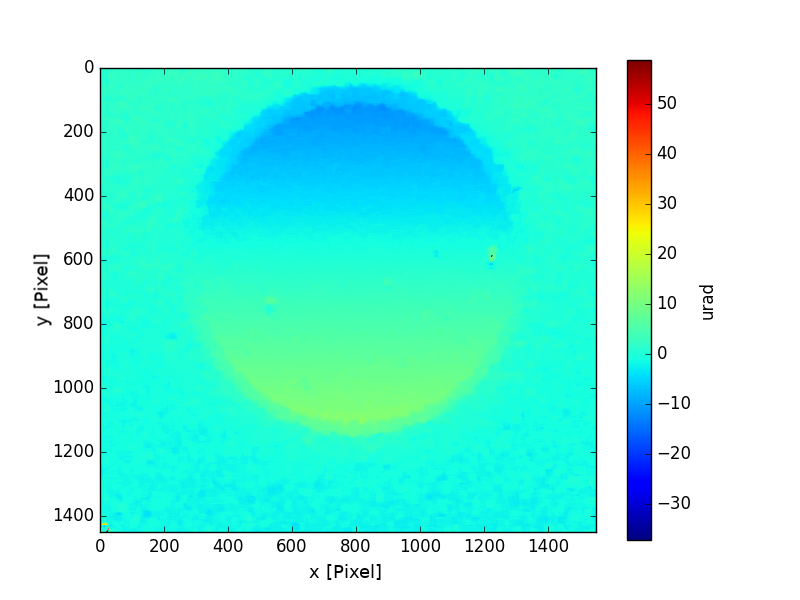
\includegraphics[width=0.38\linewidth]{img/SpeckDisV_E10001_edf_ref_start0001_1-10_edf}}};
		\only<5>{\draw[red, very thick] (-1.2, -3.5) rectangle (2.9, 3.9)};
		\only<5>{\node at (0.8, 0.5) {Horizontaler Gradient}};
		\only<5>{\node at (0.8, -3.3) {Vertikaler Gradient}};
		\only<5>{\draw[red, very thick] (-4.3, -0.3) -- (-1.2, 3.9)};
		\only<5>{\draw[red, very thick] (-4.3, -1.0) -- (-1.2, -3.5)};
		
		\only<6-7>{\node at (0.4, -2.5) {\footnote{\citeall{FC88}}};}
		\only<6-7>{\draw[red, very thick] (-6.0, -1.1) rectangle (-4.3, -1.8)};
		\only<6>{\node at (-1,0) {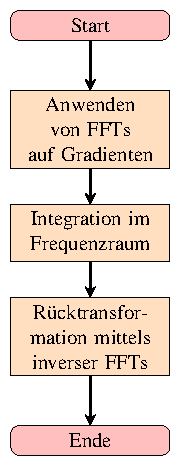
\includegraphics[width=0.17\linewidth]{pdf/graph_fc}}};
		\only<6>{\draw[red, very thick] (-4.3, -1.1) -- (-2, 2.5)};
		\only<6>{\draw[red, very thick] (-4.3, -1.8) -- (-2, -2.5)};
		\only<6>{\draw[red, very thick] (-2, -2.5) rectangle (0.0, 2.5)};
		
		\only<7>{\node at (0.5,1) {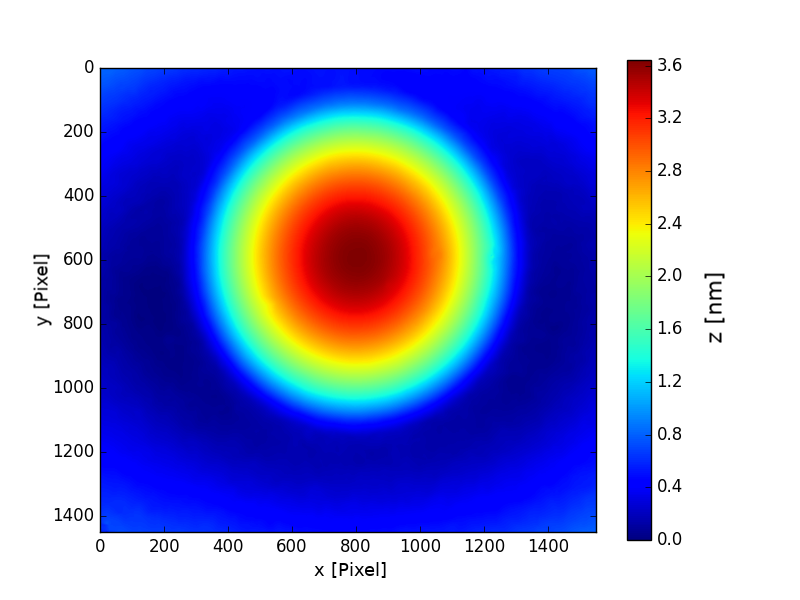
\includegraphics[width=0.6\linewidth]{img/2D_E10001_edf_ref_start0001_1-10_edf}}};
		\only<7>{\draw[red, very thick] (-2.7, -2) rectangle (3.4, 3.2)};
		\only<7>{\node at (0.7, -1.7) {Integrierte Gradientenmatrix}};
		\only<7>{\draw[red, very thick] (-4.3, -1.1) -- (-2.7, 3.2)};
		\only<7>{\draw[red, very thick] (-4.3, -1.8) -- (-2.7, -2)};
	\end{tikzpicture}
\end{frame}